\documentclass{article}
\usepackage{helvet}


\usepackage{cite}
\usepackage{amsmath,amssymb,amsfonts}
\usepackage{algorithmic}
\usepackage{graphicx}
\usepackage{textcomp}
\usepackage{xcolor}
\usepackage{hyperref}
\usepackage{placeins}
\usepackage{graphicx}
\usepackage{subcaption}



\def\BibTeX{{\rm B\kern-.05em{\sc i\kern-.025em b}\kern-.08em
    T\kern-.1667em\lower.7ex\hbox{E}\kern-.125emX}}


\title{Assignment 2: CS 754, Spring 2024-25}
\author{
\IEEEauthorblockN{
    \begin{tabular}{cccc}
        \begin{minipage}[t]{0.23\textwidth}
            \centering
            Amitesh Shekhar\\
            IIT Bombay\\
            22b0014@iitb.ac.in
        \end{minipage} & 
        \begin{minipage}[t]{0.23\textwidth}
            \centering
            Anupam Rawat\\
            IIT Bombay\\
            22b3982@iitb.ac.in
        \end{minipage} & 
        \begin{minipage}[t]{0.23\textwidth}
            \centering
            Toshan Achintya Golla\\
            IIT Bombay\\
            22b2234@iitb.ac.in
        \end{minipage} \\
        \\ 
    \end{tabular}
}
}

\date{February 16, 2025}


\usepackage{amsmath}
\usepackage{amssymb}
\usepackage{hyperref}
\usepackage{ulem,graphicx}
\usepackage[margin=0.5in]{geometry}

\begin{document}
\maketitle

\\
\\

\textbf{Declaration:} The work submitted is our own, and
we have adhered to the principles of academic honesty while completing and submitting this work. We have not
referred to any unauthorized sources, and we have not used generative AI tools for the work submitted here.

\begin{enumerate}
\item Your task here is to implement the ISTA algorithm:
\begin{enumerate}
\item Consider the `Barbara' image from the homework folder. Add iid Gaussian noise of mean 0 and variance 4 (on a [0,255] scale) to it, using the `randn' function in MATLAB. Thus $\boldsymbol{y} = \boldsymbol{x} + \boldsymbol{\eta}$ where $\boldsymbol{\eta} \sim \mathcal{N}(0,4)$. You should obtain $\boldsymbol{x}$ from $\boldsymbol{y}$ using the fact that patches from $\boldsymbol{x}$ have a sparse or near-sparse representation in the 2D-DCT basis. 
\item Divide the image shared in the homework folder into patches of size $8 \times 8$. Let $\boldsymbol{x_i}$ be the vectorized version of the $i^{th}$ patch. Consider the measurement $\boldsymbol{y_i} = \boldsymbol{\Phi x_i}$ where $\boldsymbol{\Phi}$ is a $32 \times 64$ matrix with entries drawn iid from $\mathcal{N}(0,1)$. Note that $\boldsymbol{x_i}$ has a near-sparse representation in the 2D-DCT basis $\boldsymbol{U}$ which is computed in MATLAB as `kron(dctmtx(8)',dctmtx(8)')'. In other words, $\boldsymbol{x_i} = \boldsymbol{U \theta_i}$ where $\boldsymbol{\theta_i}$ is a near-sparse vector. Your job is to reconstruct each $\boldsymbol{x_i}$ given $\boldsymbol{y_i}$ and $\boldsymbol{\Phi}$ using ISTA. Then you should reconstruct the image by averaging the overlapping patches. You should choose the $\alpha$ parameter in the ISTA algorithm judiciously. Choose $\lambda = 1$ (for a [0,255] image). Display the reconstructed image in your report. State the RMSE given as $\|X(:)-\hat{X}(:)\|_2/\|X(:)\|_2$ where $\hat{X}$ is the reconstructed image and $X$ is the true image. Repeat this with the `goldhill' image (take the top-left portion of size 256 by 256 only). \textsf{[12 points]}
\item Implement both the above cases using the FISTA algorithm from the research paper \url{https://epubs.siam.org/doi/10.1137/080716542}. \textsf{[12 points]}
\item Read the research paper and explain in which precise mathematical sense the FISTA algorithm is faster than ISTA. Also, why is it faster than ISTA? \textsf{[12 points]}
\end{enumerate}
\makebox[0pt][l]{\hspace{-7pt}\textit{Soln:}}
\begin{enumerate}
    \item The Original and Noisy images(Gaussian noise of mean 0 and variance 4 was added) as as follows:
\FloatBarrier
\begin{figure}[!h]
    \centering
    \begin{subfigure}[b]{0.45\textwidth}
        \centering
        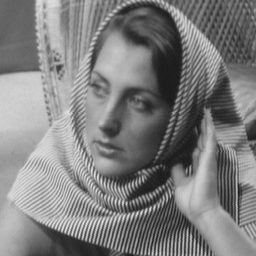
\includegraphics[width=0.6\textwidth]{HomeWork_2/2/images/barbara256.png}
        \caption{Original Barbara}
    \end{subfigure}
    \begin{subfigure}[b]{0.45\textwidth}
        \centering
        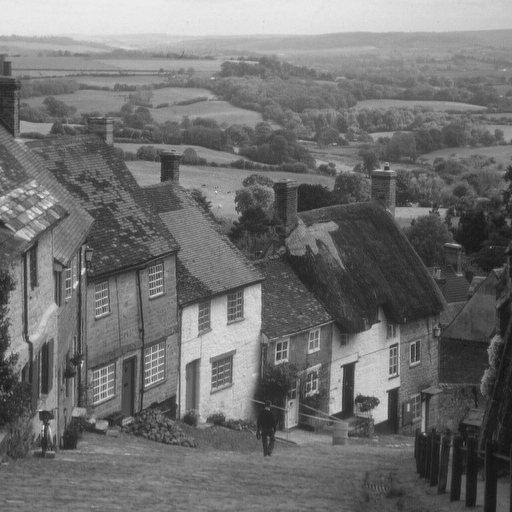
\includegraphics[width=0.6\textwidth]{HomeWork_2/2/images/goldhill.png}
        \caption{Original Goldhill}
    \end{subfigure}
    \caption{Original Images}
\end{figure}

\begin{figure}[!h]
    \centering
    \begin{subfigure}[b]{0.45\textwidth}
        \centering
        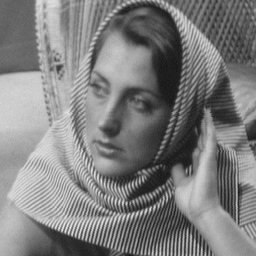
\includegraphics[width=0.6\textwidth]{HomeWork_2/2/images/Noisy_Barbara.png}
        \caption{Noisy Barbara}
    \end{subfigure}
    \begin{subfigure}[b]{0.45\textwidth}
        \centering
        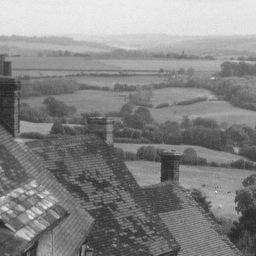
\includegraphics[width=0.6\textwidth]{HomeWork_2/2/images/Noisy_Goldhill.png}
        \caption{Noisy Goldhill}
    \end{subfigure}
    \caption{Noisy Images}
\end{figure}
\FloatBarrier
\item The results of the ISTA reconstruction algorithm are as follows:
\begin{figure}[!h]
    \centering
    \begin{subfigure}[b]{0.45\textwidth}
        \centering
        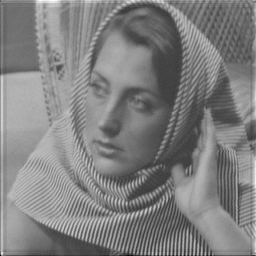
\includegraphics[width=0.6\textwidth]{HomeWork_2/2/images/Reconstructed_Barbara_ISTA.png}
        \caption{Reconstructed Barbara(RMSE = 0.14021)}
    \end{subfigure}
    \begin{subfigure}[b]{0.45\textwidth}
        \centering
        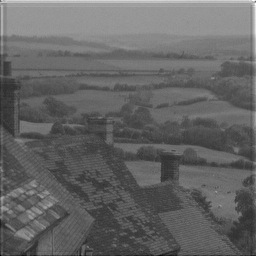
\includegraphics[width=0.6\textwidth]{HomeWork_2/2/images/Reconstructed_Goldhill_ISTA.png}
        \caption{Reconstructed Goldhill(RMSE = 0.28694)}
    \end{subfigure}
    \caption{Results of ISTA}
\end{figure}
\item The results of the FISTA reconstruction algorithm are as follows:
\begin{figure}[!h]
    \centering
    \begin{subfigure}[b]{0.45\textwidth}
        \centering
        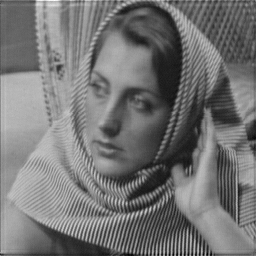
\includegraphics[width=0.6\textwidth]{HomeWork_2/2/images/Reconstructed_Barbara_FISTA.png}
        \caption{Reconstructed Barbara(RMSE = 0.10436)}
    \end{subfigure}
    \begin{subfigure}[b]{0.45\textwidth}
        \centering
        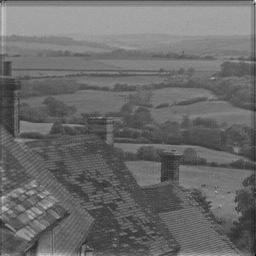
\includegraphics[width=0.6\textwidth]{HomeWork_2/2/images/Reconstructed_Goldhill_FISTA.png}
        \caption{Reconstructed Goldhill(RMSE = 0.26047)}
    \end{subfigure}
    \caption{Results of FISTA}
\end{figure}
\item 
The Fast Iterative Shrinkage-Thresholding Algorithm (FISTA) provides a significant improvement over the standard Iterative Shrinkage-Thresholding Algorithm (ISTA) in terms of convergence speed. The primary reason for this acceleration is the incorporation of a momentum term inspired by Nesterov's acceleration method.
\\
As explained in the paper, the convergence rate of ISTA is given by:
\begin{equation}
    F(x_k) - F(x^*) \leq \mathcal{O}\left(\frac{1}{k}\right),
\end{equation}

On the other hand, FISTA achieves a much faster convergence rate:
\begin{equation}
    F(x_k) - F(x^*) \leq \mathcal{O}\left(\frac{1}{k^2}\right).
\end{equation}
where \( F(x) \) is the objective function, and \( x^* \) is the optimal solution.
This improvement implies that for the same number of iterations, FISTA gets significantly closer to the optimal solution than ISTA.
\\\\
How do we explain this? The key idea behind FISTA's acceleration is the introduction of a momentum term that modifies the update step. Instead of using only the current iterate \( x_k \), FISTA computes an auxiliary sequence \( y_k \) as a linear combination of the current and previous iterates. For explanation using equations, consider the following: \\Both ISTA and FISTA rely on the proximal operator \( p_L(y) \), which is defined as:
\begin{equation}
    p_L(y) = \arg\min_x \left\{ f(y) + \langle x - y, \nabla f(y) \rangle + \frac{L}{2} \|x - y\|^2 + g(x) \right\}.
\end{equation}
Here, \( p_L(y) \) finds the next iterate by combining a gradient descent step and a shrinkage/thresholding operation.

- In ISTA, the update is performed as:
  \begin{equation}
      x_{k+1} = p_L(x_k)
  \end{equation}
  This means each step moves in the gradient direction while applying a thresholding operation.

- In FISTA, instead of applying \( p_L \) directly to \( x_k \), an intermediate variable \( y_k \) is introduced to accelerate convergence:
  \begin{equation}
      x_{k+1} = p_L(y_k)
  \end{equation}
  \begin{equation}
      t_{k+1} = \frac{1 + \sqrt{1 + 4t_k^2}}{2}
  \end{equation}
  \begin{equation}
      y_k = x_k + \frac{t_k - 1}{t_{k+1}} (x_k - x_{k-1})
  \end{equation}
Calculating the momentum as shown above allows FISTA to "leap" forward in the optimization landscape, reducing the number of iterations required to reach a given accuracy. \\
FISTA is slightly more computationally expensive per iteration, but the faster convergence often makes it more efficient overall. Therefore, due to the improved convergence rate, FISTA is more efficient than ISTA in practical applications, particularly in image reconstruction and compressed sensing problems. The reduced number of iterations translates to significant computational savings while preserving the simplicity of ISTA. \\
In summary, in most practical scenarios, FISTA is the preferred choice due to its accelerated convergence and efficiency, although ISTA is simpler to implement and slightly more robust, making it a good choice for small-scale problems or when implementation simplicity is a priority.

\end{enumerate}
\end{enumerate}
\end{document}
